\section{Section: Prelude}

\section{Section Intro}

\begin{frame}{About us}
  \begin{columns}[fullwidth,T]
    \hspace*{.25\LeftSlideIndent}%
    \begin{column}{.4\linewidth}
      \centering
      \small
      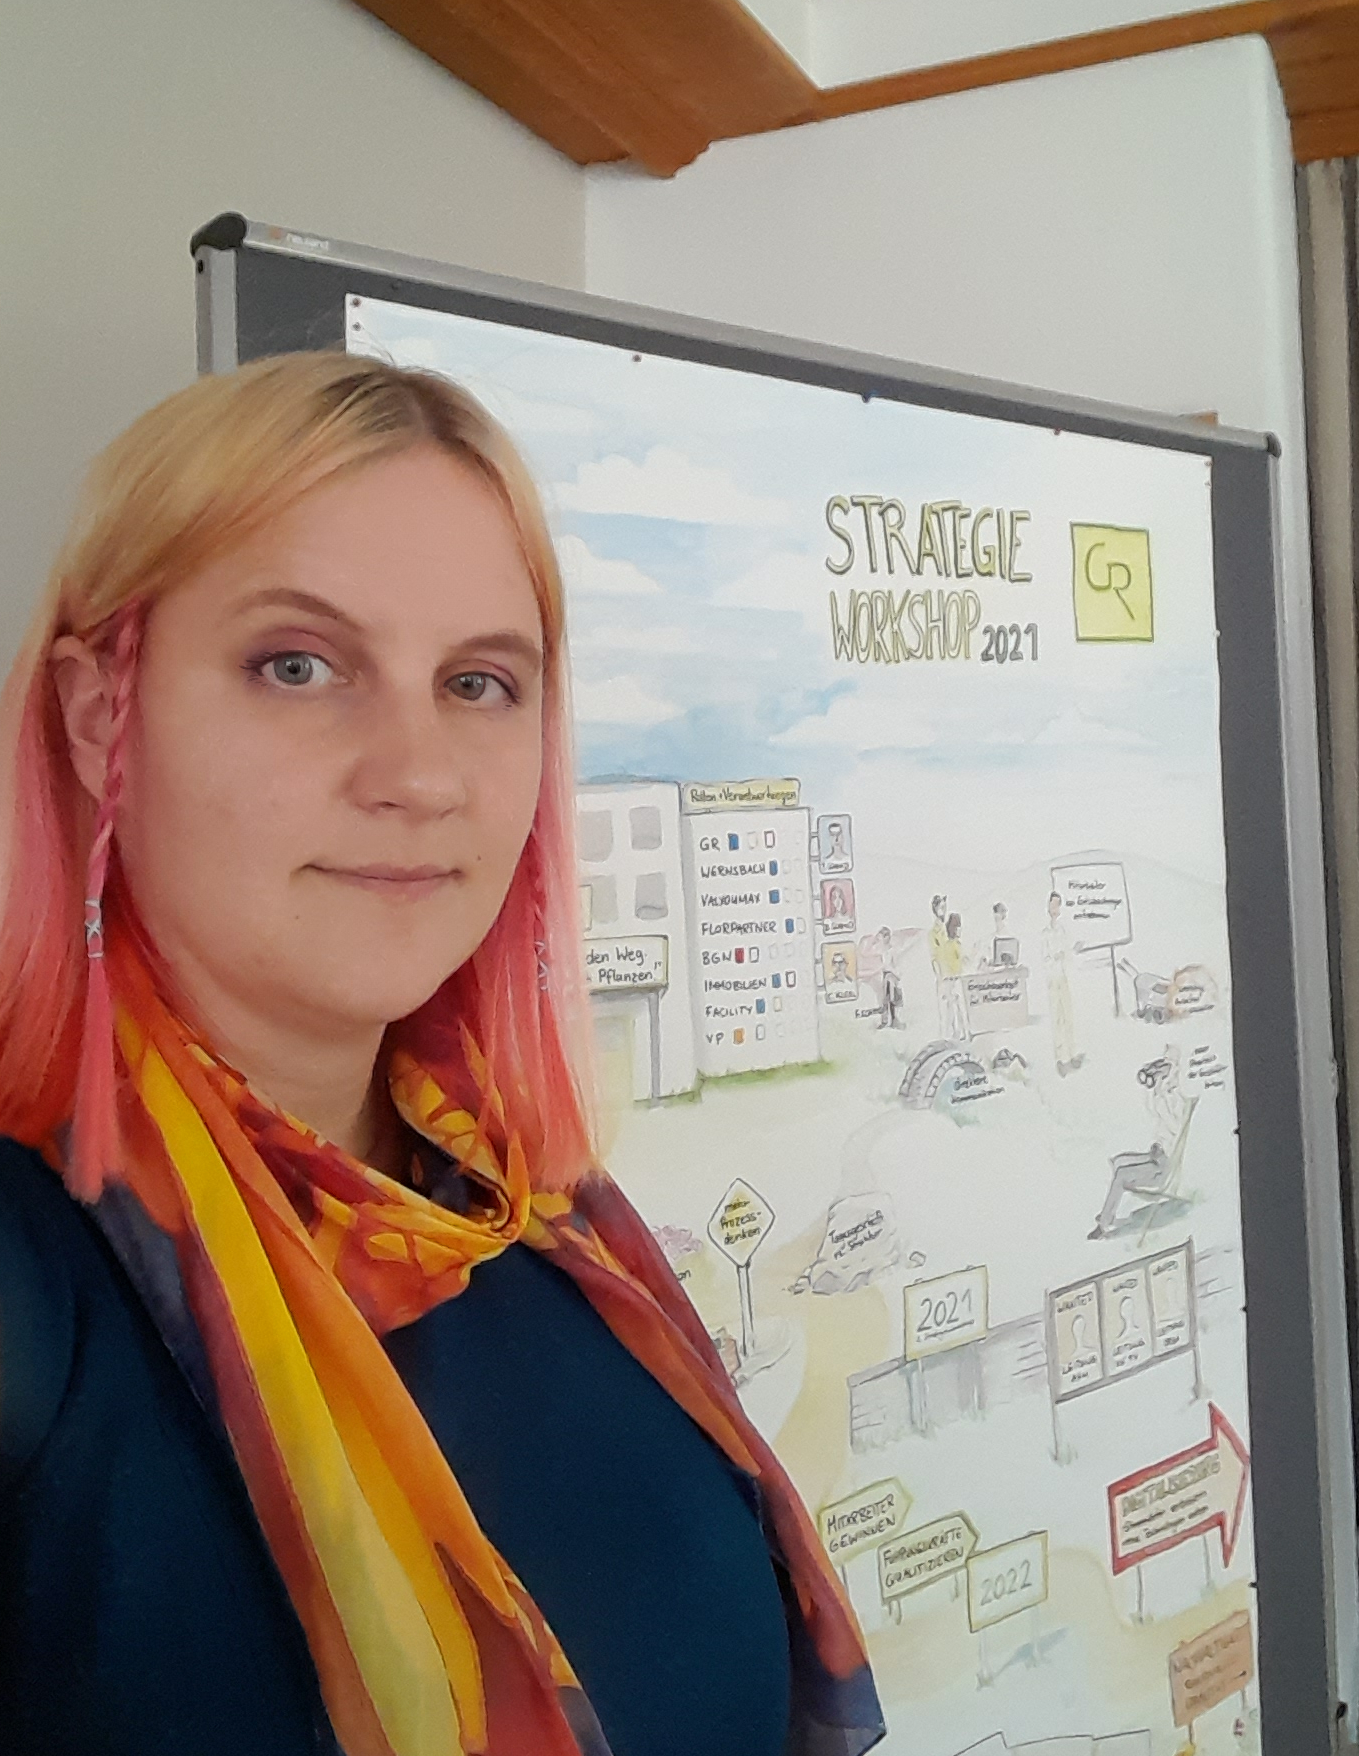
\includegraphics[width=.78\linewidth,trim=0 60 0 220,clip]{graphics/mullana.jpg}
      \\ Scientific Illustration: \\ Lisa (mullana) Schmidt
    \end{column}
    \begin{column}{\dimexpr.6\linewidth-.25\LeftSlideIndent}
      \small
      \vspace{-0.6em}
      \begin{itemize}
        \item Karolin Varner: Managing Directory/Lead Scientist of Rosenpass e. V.
        \item Rose Turing: Student at TU Munich who helped create this talk and who will give a portion of it
        \item Rosenpass e. V. is at the intersection of science, business, and infrastructure
        \item \textbf{Research}: Cryptography, protocol design, key exchanges
        \item \textbf{Product}: Rosenpass, which upgrades the WireGuard VPN to post-quantum security
        \item \textbf{Focus}: Making cryptography approachable. How to think about the technology?
      \end{itemize}
    \end{column}%
  \end{columns}
\end{frame}
